% !TEX encoding = UTF-8 Unicode
\documentclass[10pt,usepdftitle=false,aspectratio=169]{beamer}
\usepackage[left]{muibkitsec}
\usepackage{listings}

\usepackage{microtype}
\usepackage{graphbox}
\usepackage{booktabs} 
\usepackage{tikz-cd}
\usepackage{amsmath,amssymb,amsfonts,amsthm,mathtools}
\usepackage{algorithmic}
\usepackage{textcomp}
\usepackage{xcolor}
\usepackage{diagbox}
\usepackage{float, multirow}
\usepackage{tikz, pgfplots}
\usepackage{tikzsymbols}
\usetikzlibrary{spy}
\usepackage{subcaption}
\usepgfplotslibrary{groupplots}
\pgfplotsset{compat=newest}

% ------------------------------------------------------------------------
\title{Adversarial Label Flips}
\author{Matthias Dellago \& Maximilian Samsinger}
\date{10 June 2021}

% ------------------------------------------------------------------------

\begin{document}
\DeclarePairedDelimiter\abs{\lvert}{\rvert}%
\DeclarePairedDelimiter\norm{\lVert}{\rVert}%
\DeclarePairedDelimiter\ceil{\lceil}{\rceil}
\DeclarePairedDelimiter\floor{\lfloor}{\rfloor}

\begin{frame}[plain]
	\maketitle
\end{frame}	

\begin{frame}[plain]
	\huge A short recap
\end{frame}	


\begin{frame}[noframenumbering,fragile]
	\frametitle{Adversarial attack}
	\begin{tabular}{ccccc}
		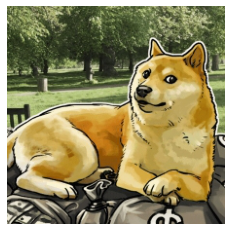
\includegraphics[align=c,width=0.28\columnwidth]{plots/original_04282.png} & \Huge{+} & \Huge{\textbf{$\epsilon$}}\ 
\includegraphics[align=c,width=0.28\columnwidth]{plots/difference_amplified_by_50.png}\ & \Huge{=} & 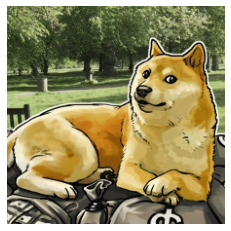
\includegraphics[align=c,width=0.28\columnwidth]{plots/adversarial_09999.png} \\~\\
		\huge{Husky} &&\qquad \large{Noise (PGD-40)}&& \huge{Handkerchief} \\
		(42.82\% confidence) && \qquad 50x amplified && (99.999988\% confidence) 
	\end{tabular}
	\source{Source: \url{ctf.codes}, circa 2021}
\end{frame}

\begin{frame}[fragile]
	\frametitle{What we want to do}
	\begin{block}{Confusion Matrix}
		\begin{table}
			\setlength{\extrarowheight}{2pt}
			\begin{tabular}{cc|c|c|c|}
				& \multicolumn{1}{c}{} & \multicolumn{3}{c}{Categorised as}\\
				& \multicolumn{1}{c}{} & \multicolumn{1}{c}{Dog}  & \multicolumn{1}{c}{Cat} & \multicolumn{1}{c}{Plane} \\\cline{3-5}
				\multirow{3}*{Adversarial Example of a}  & Dog & 0.0 & ? & ?\\\cline{3-5}
				& Cat & ? & 0.0 &  ? \\\cline{3-5}
				& Plane & ? & ? &  0.0 \\\cline{3-5}
			\end{tabular}
		\end{table}
		How many modified dogs get classified as cats vs as planes? etc.
	\end{block}
\end{frame}

\begin{frame}[plain]
	\huge Some simple theory
\end{frame}	

\begin{frame}[plain]
	\large We want similar images that are classified differently.\\
	But what is "similar"?
\end{frame}	

\begin{frame}[fragile]
	\frametitle{Quantifying Difference ($\epsilon$)}

	\begin{tabular}{cccc}
		
	$L^0$-Norm & 	$L^1$-Norm & 	$L^2$-Norm & 	$L^\infty$-Norm \vspace{5pt} \\
	
	
	
	\shortstack{Number of \\ different pixels} & \shortstack{Sum of \\ all differences} & \shortstack{Sum of the $square$ \\ of all differences} & \shortstack{Maximum of \\ all differences} \\
	
	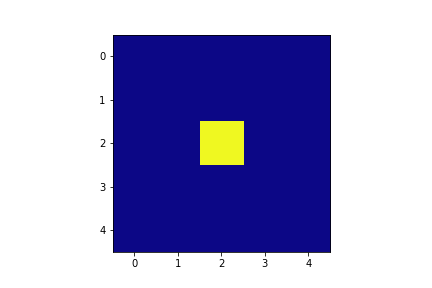
\includegraphics[align=c,width=0.3\columnwidth]{plots/L0.png} &
	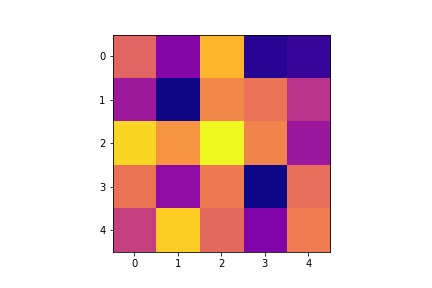
\includegraphics[align=c,width=0.3\columnwidth]{plots/L1.png} &
	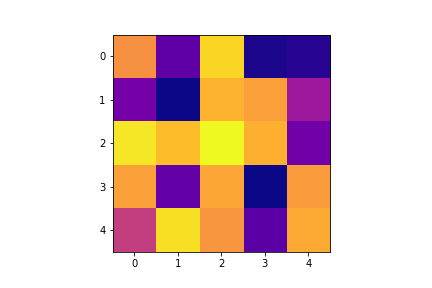
\includegraphics[align=c,width=0.3\columnwidth]{plots/L2.png} &
	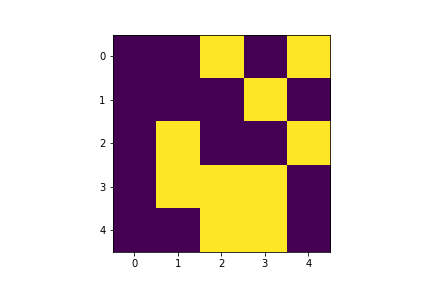
\includegraphics[align=c,width=0.3\columnwidth]{plots/Linf.png} 
	\\
	
	\shortstack{Change very few \\ pixels maximally}&Minimise sum&\shortstack{Minimise sum \\ of squares}&\shortstack{Change all \\ pixels equally}
	\end{tabular}
\end{frame}


\begin{frame}[fragile]
	\frametitle{Two Different Approaches}
	\begin{tikzcd}[column sep=4em]
		& \shortstack{small difference and \\ big misclassification} \\
		\text{small difference} \arrow{ur}{ \text{maximise misclassification} } && \text{big misclassification} \arrow[ul, "\text{minimise difference}"']
	\end{tikzcd}
\end{frame}

\begin{frame}[fragile]
	\frametitle{Projected Gradient Decent}
	\begin{columns}
		\begin{column}{.5\columnwidth}
			\begin{enumerate}
				\item Pick spot in epsilon ball
				\item Iterate gradient decent
				\item If leaving ball, project back onto surface
				\item Repeat to convergence
			\end{enumerate}
			
		\end{column}

		\begin{column}{.5\columnwidth}
			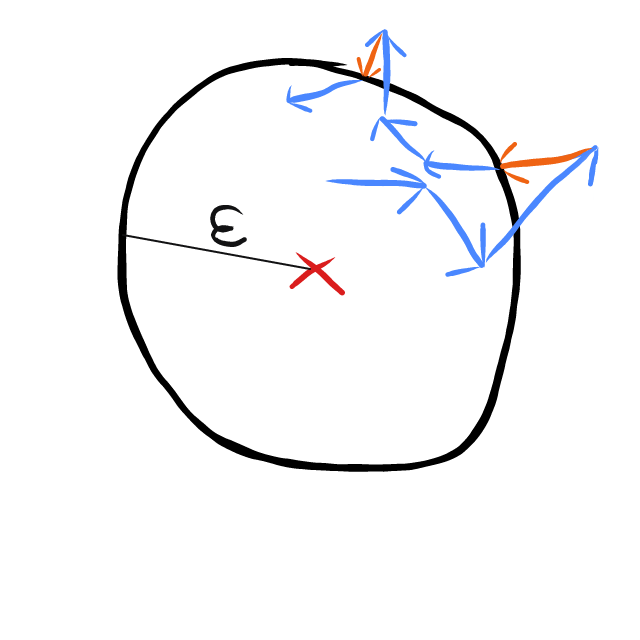
\includegraphics[width= \textwidth]{plots/pgd_sketch.png}
		\end{column}
	\end{columns}

	\source{Towards Deep Learning Models Resistant to Adversarial Attacks, Aleksander Madry et al., arXiv, 2019}
\end{frame}


\begin{frame}[fragile]
	\frametitle{Projected Gradient Decent}
	
	\begin{center}
		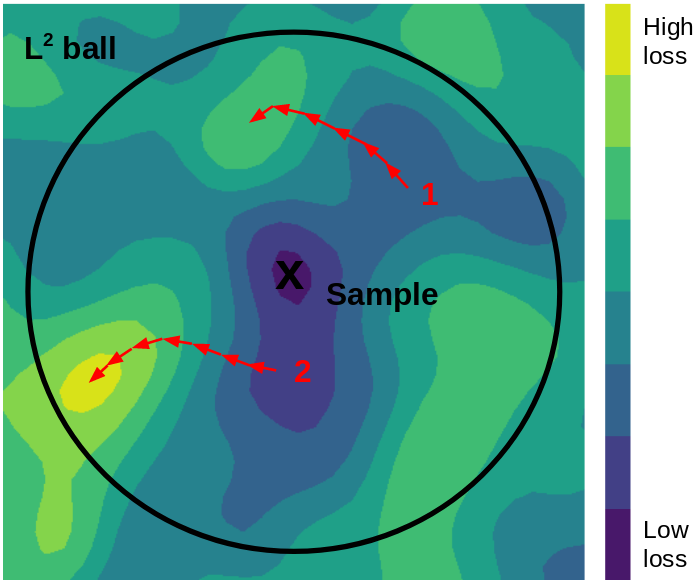
\includegraphics[height=0.75 	\textheight]{plots/pgd_pic.png}
	\end{center}

	\source{Know your enemy, Oscar Knagg, towardsdatascience.com, 2019}
\end{frame}


\begin{frame}[fragile]
	\frametitle{Carlini-Wagner-Attack}
	
	\large Original approach: minimise difference while always staying in "misclassification territory". \\
	
	\medskip
	Problem: Non-linearity of constraint makes optimimisation difficult.
	
	\source{Towards Evaluating the Robustness of Neural Networks, Nicholas Carlini and David Wagner, IEEE, 2017}
\end{frame}

\begin{frame}[fragile]
	\frametitle{Carlini-Wagner-Attack}
	
	\large Solution: Pack constraint into the function that is optimised.\\
	
	\bigskip
	
	$\rightarrow$ minimise: difference - "how misclassified is x?"*\\
	\smallskip
	
	i.e. minimise difference while maximising misclassification.\\
	\bigskip
	
	Apply Adam optimisation.
	
	\source{*loss function\\
	\smallskip
	Towards Evaluating the Robustness of Neural Networks, Nicholas Carlini and David Wagner, IEEE, 2017}
\end{frame}

\begin{frame}
	\huge Code
\end{frame}

\begin{frame}
	\huge Results
\end{frame}

\begin{frame}
	\frametitle{MNIST, $L^\infty$-PGD}
	\begin{tabular}{cccc}
		
		$\epsilon = 0.01$  & 	$\epsilon = 0.02$ & 	$\epsilon = 0.05$ & 	$\epsilon = 0.1$ \\
		
		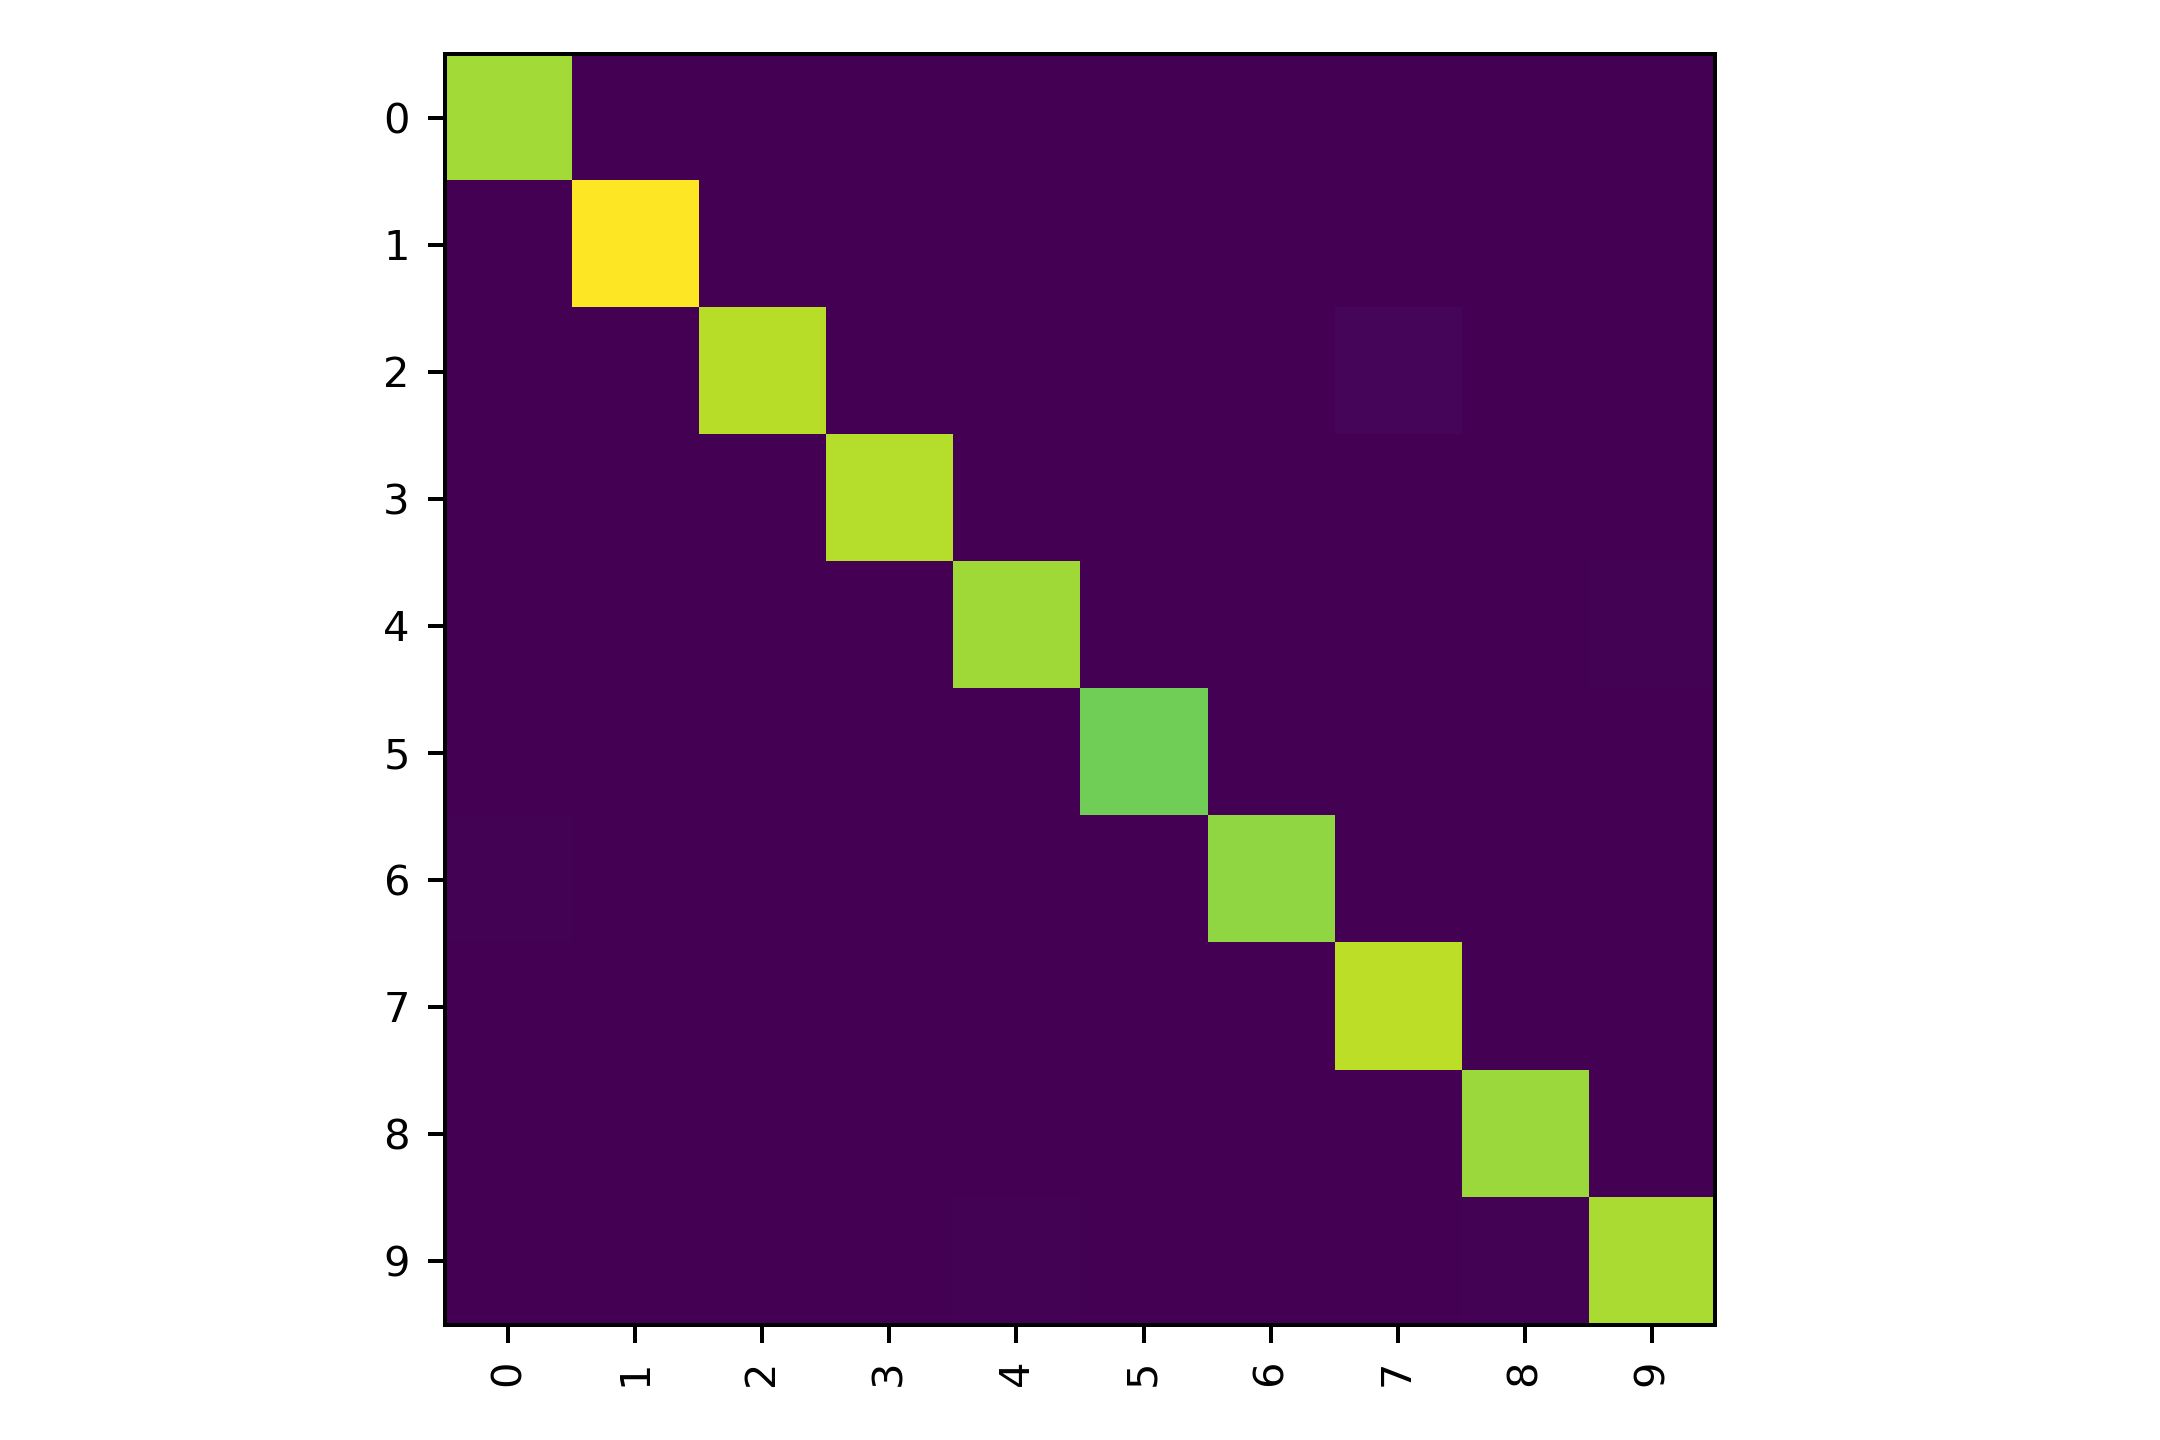
\includegraphics[align=c,width=0.3\columnwidth]{../code/results/MNIST/figures/LinfPGD, epsilon=0.01.png} &
		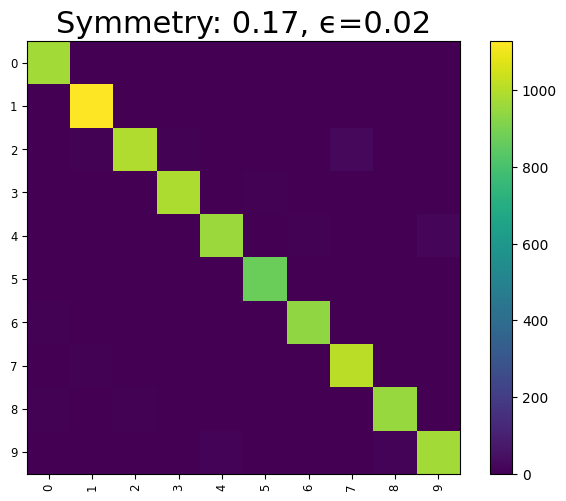
\includegraphics[align=c,width=0.3\columnwidth]{../code/results/MNIST/figures/LinfPGD, epsilon=0.02.png} &
		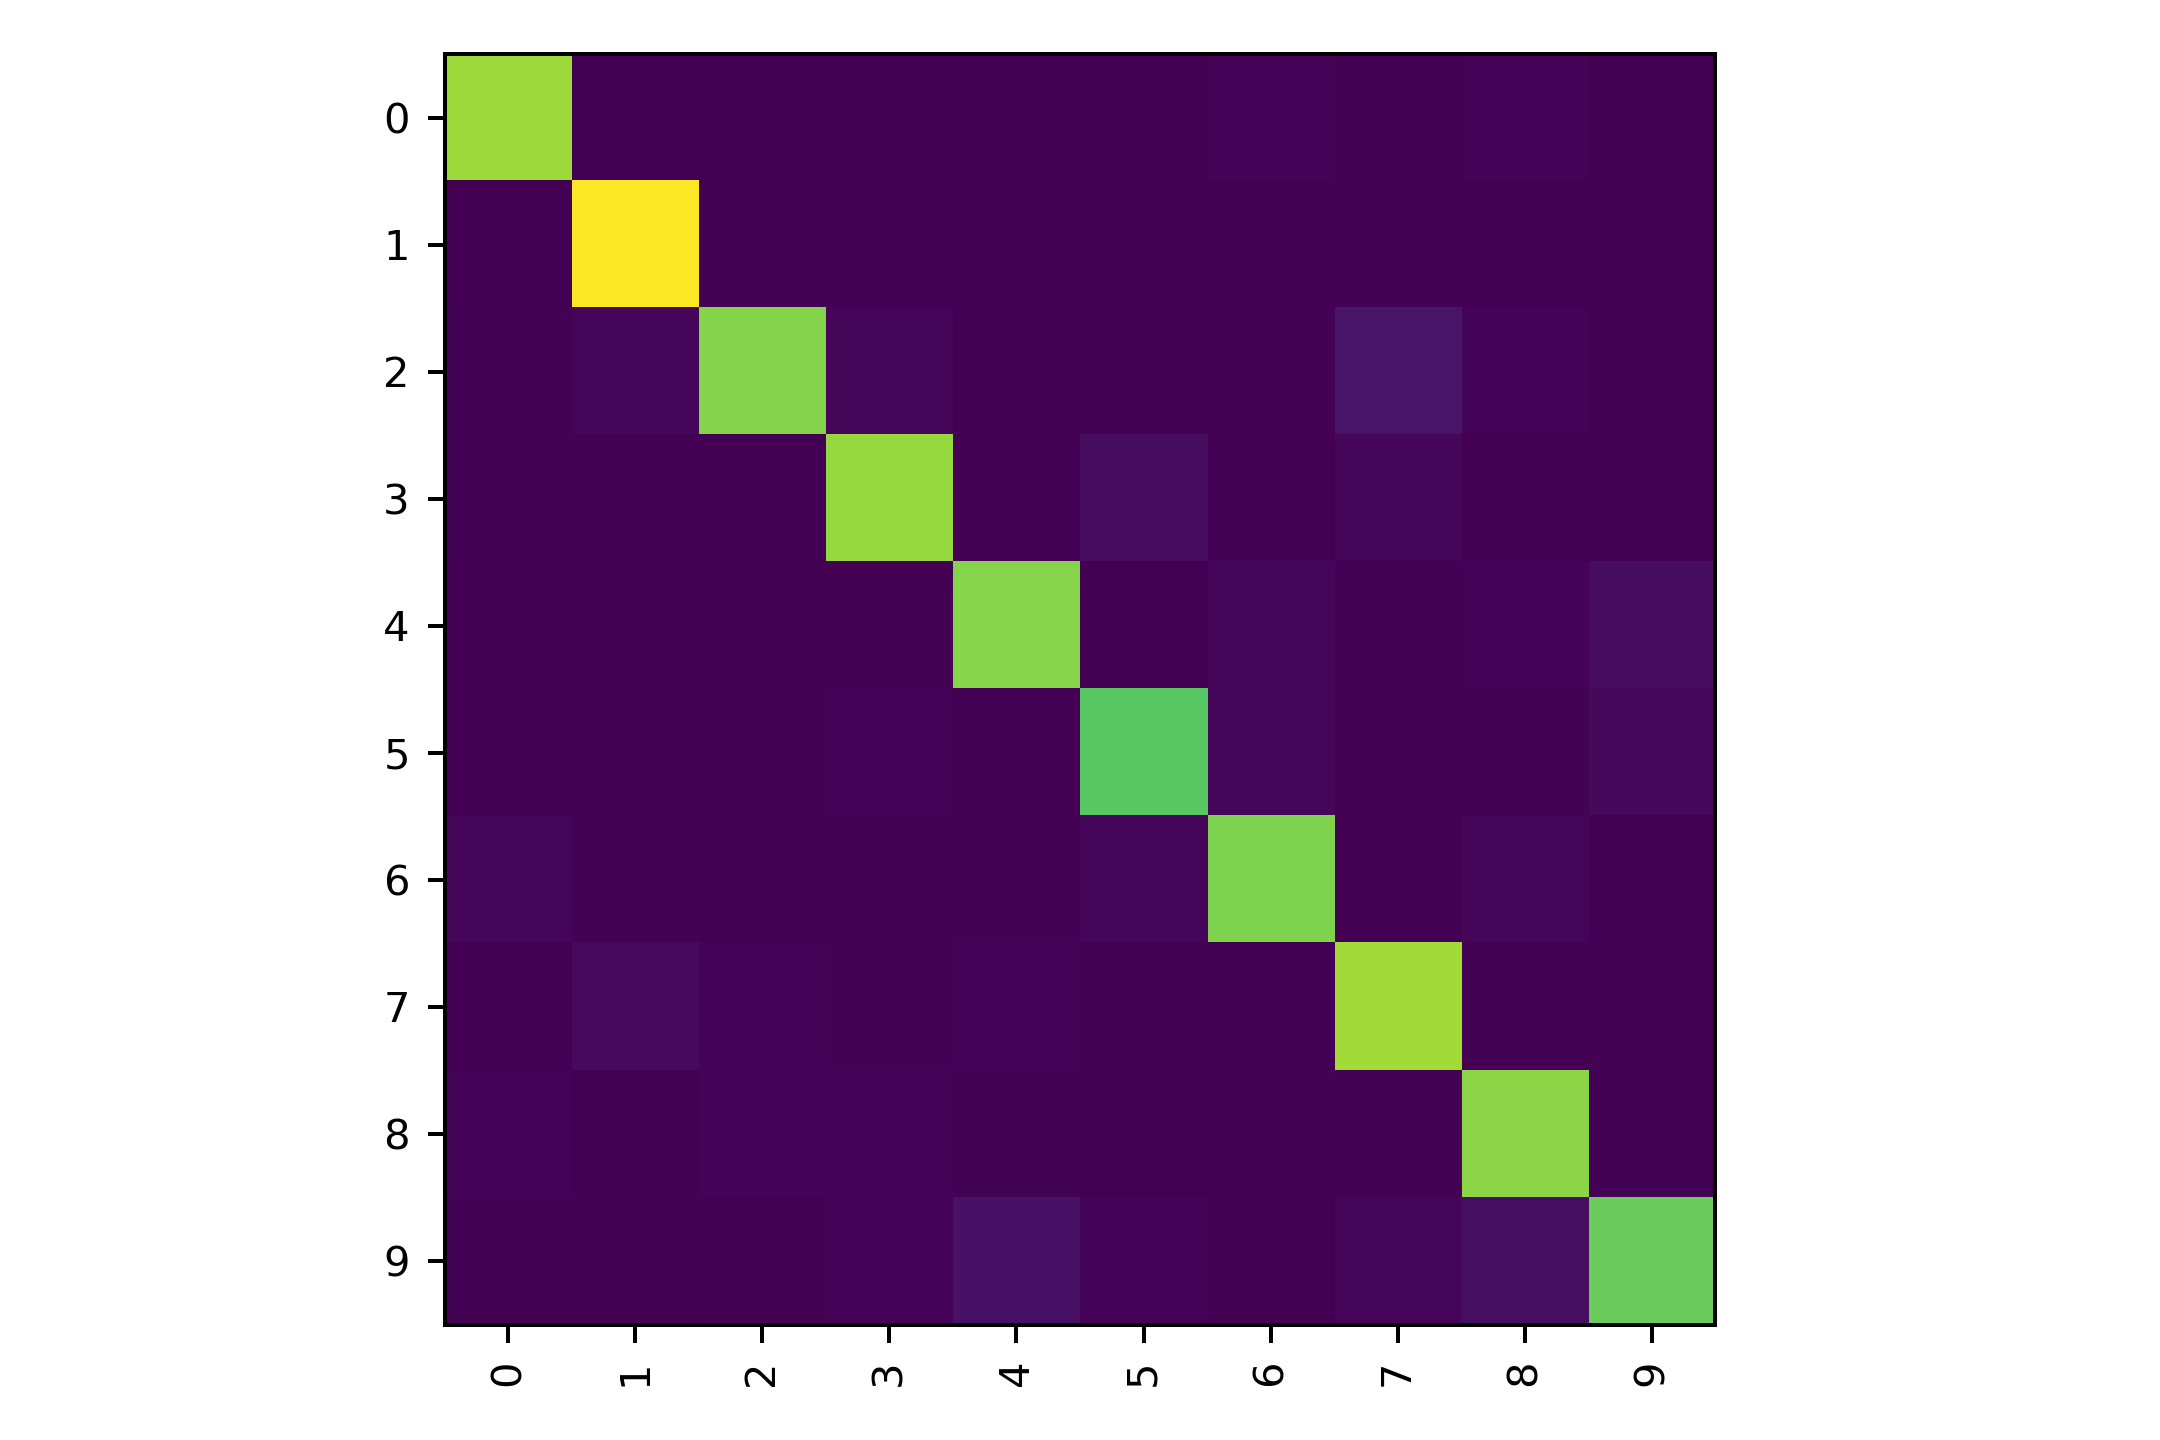
\includegraphics[align=c,width=0.3\columnwidth]{../code/results/MNIST/figures/LinfPGD, epsilon=0.05.png} &
		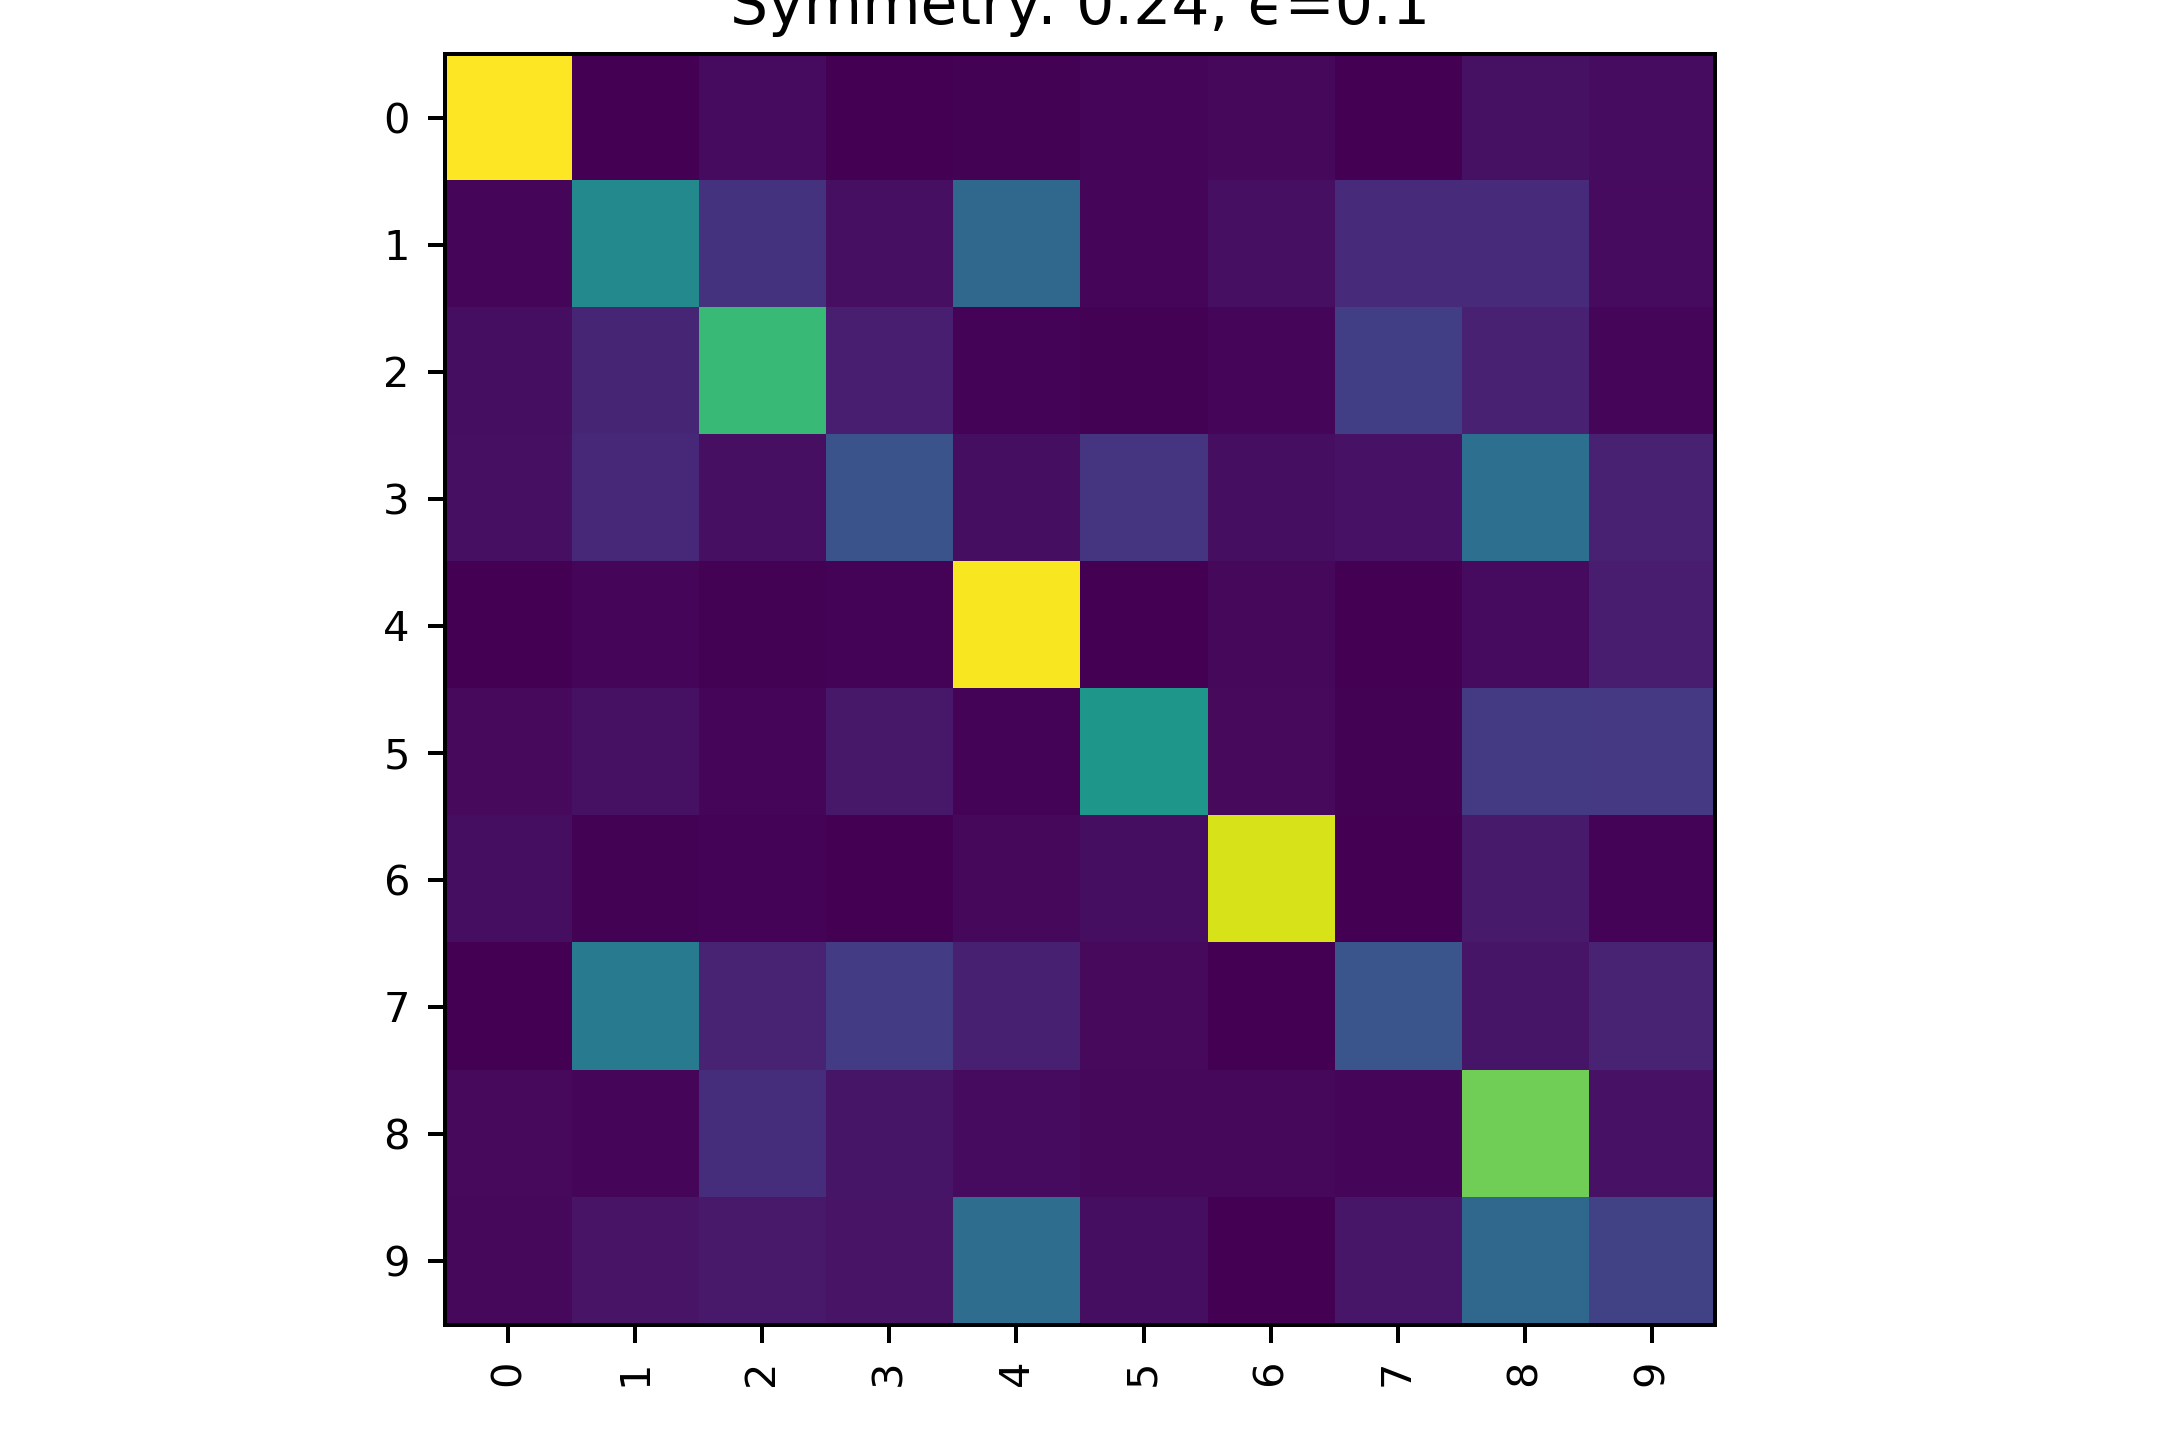
\includegraphics[align=c,width=0.3\columnwidth]{../code/results/MNIST/figures/LinfPGD, epsilon=0.1.png} 
		\bigskip \\
		
		$\epsilon = 0.2$  & 	$\epsilon = 0.5$ & 	$\epsilon = 1$ & \\
		
		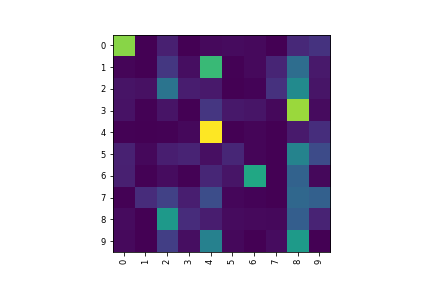
\includegraphics[align=c,width=0.3\columnwidth]{../code/results/MNIST/figures/LinfPGD, epsilon=0.2.png} &
		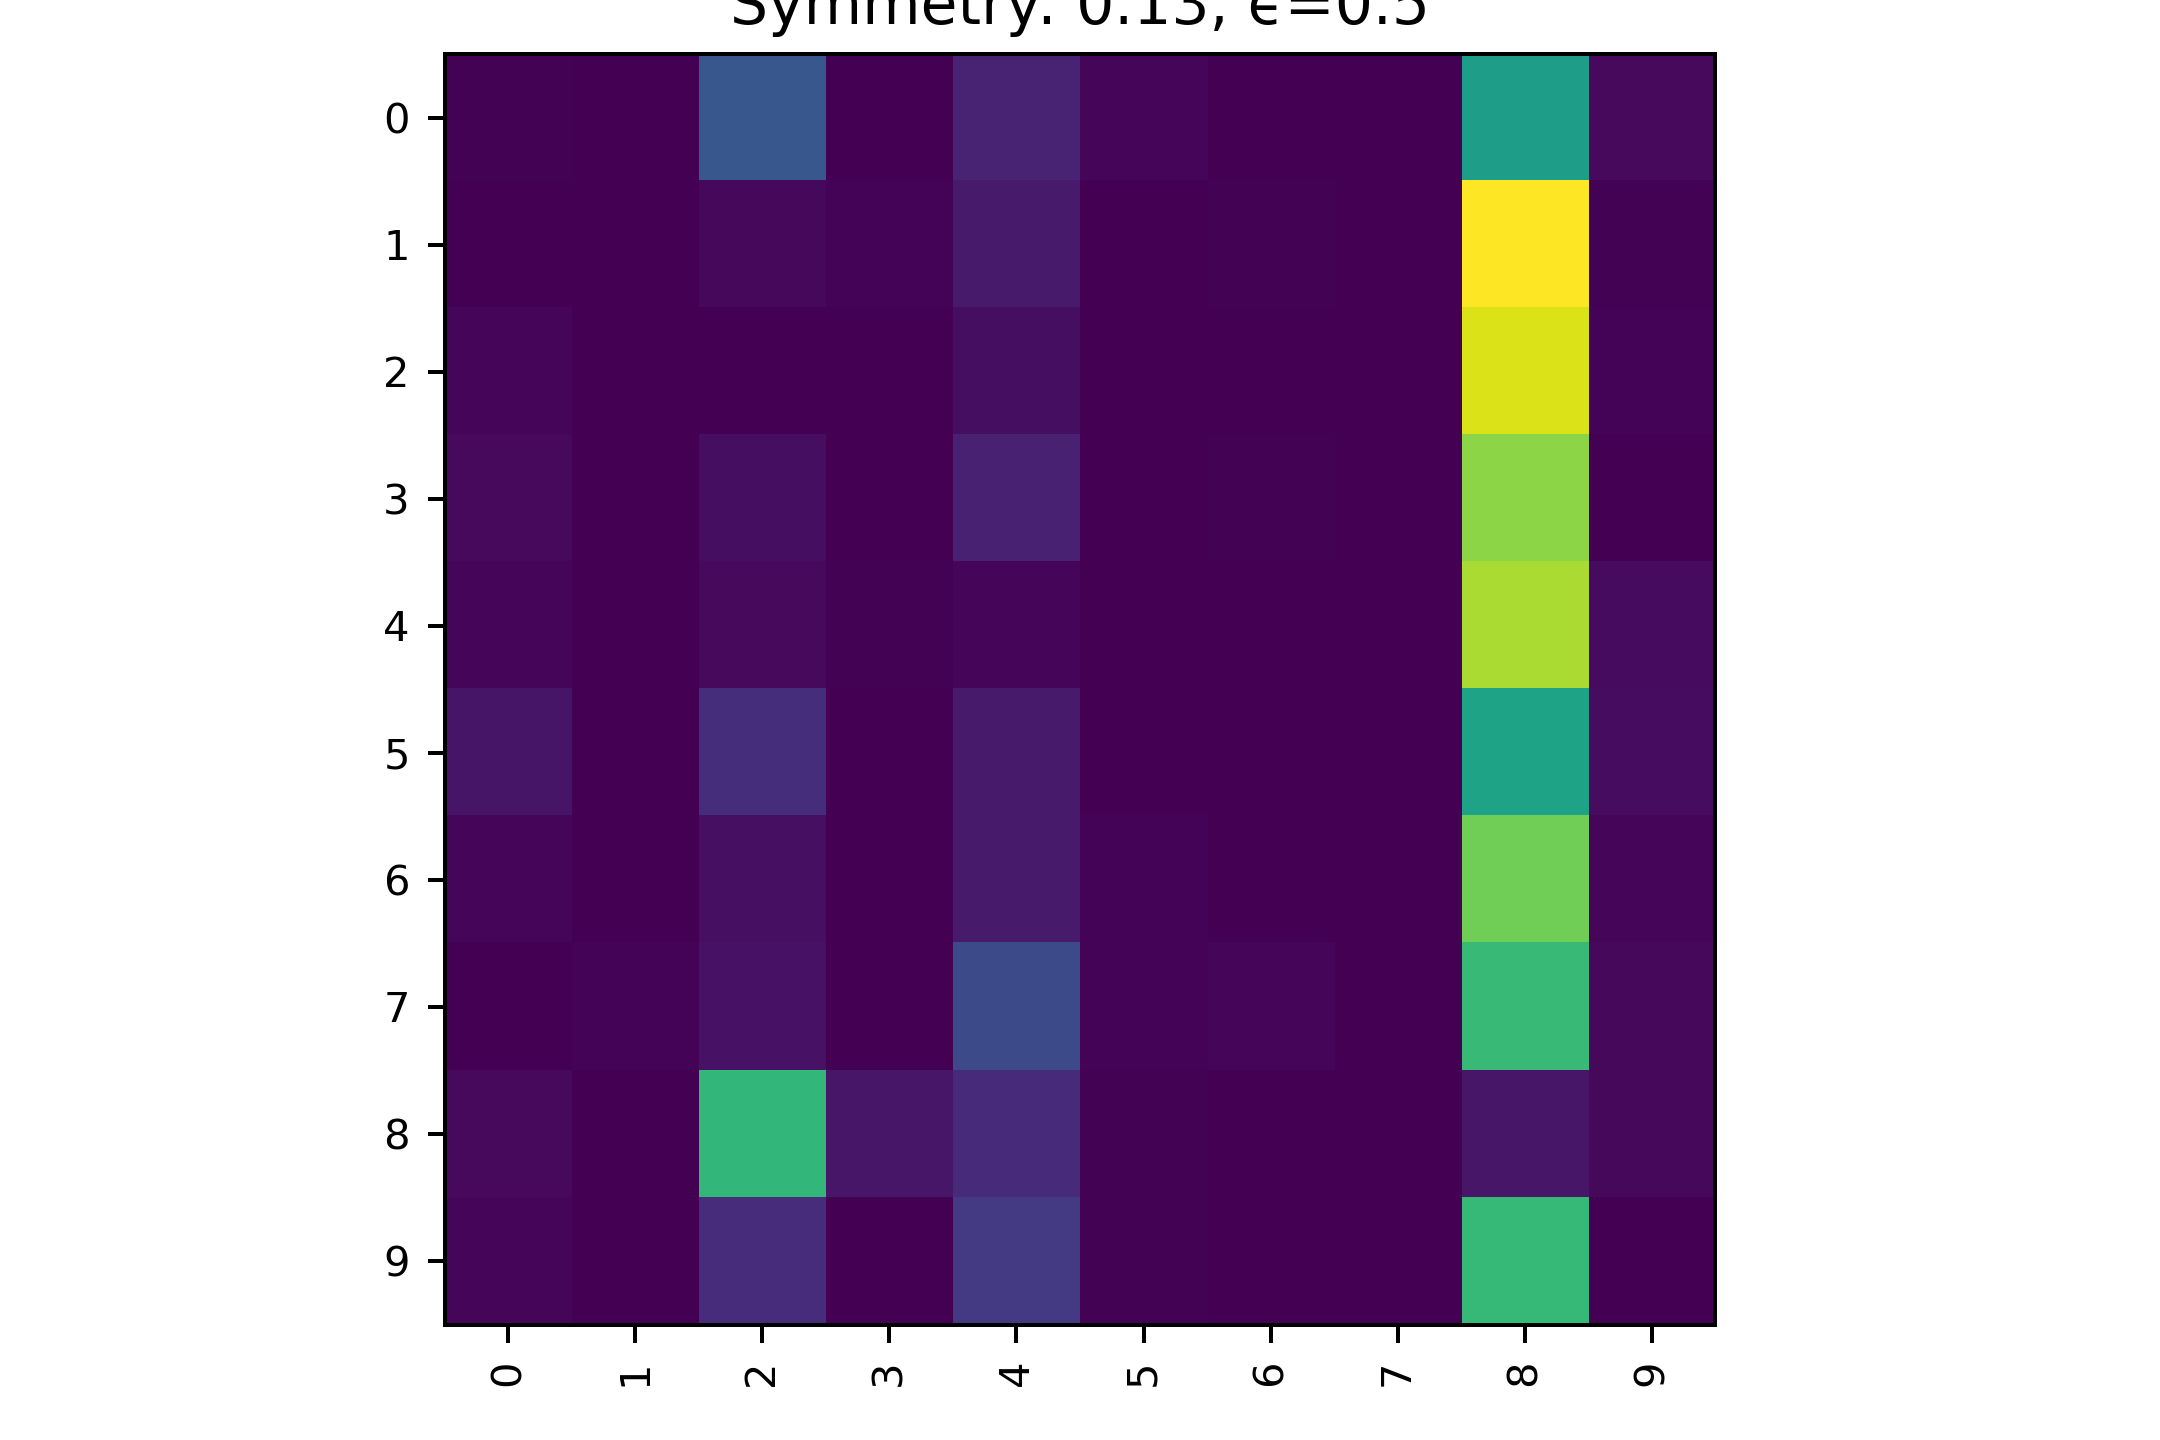
\includegraphics[align=c,width=0.3\columnwidth]{../code/results/MNIST/figures/LinfPGD, epsilon=0.5.png} &
		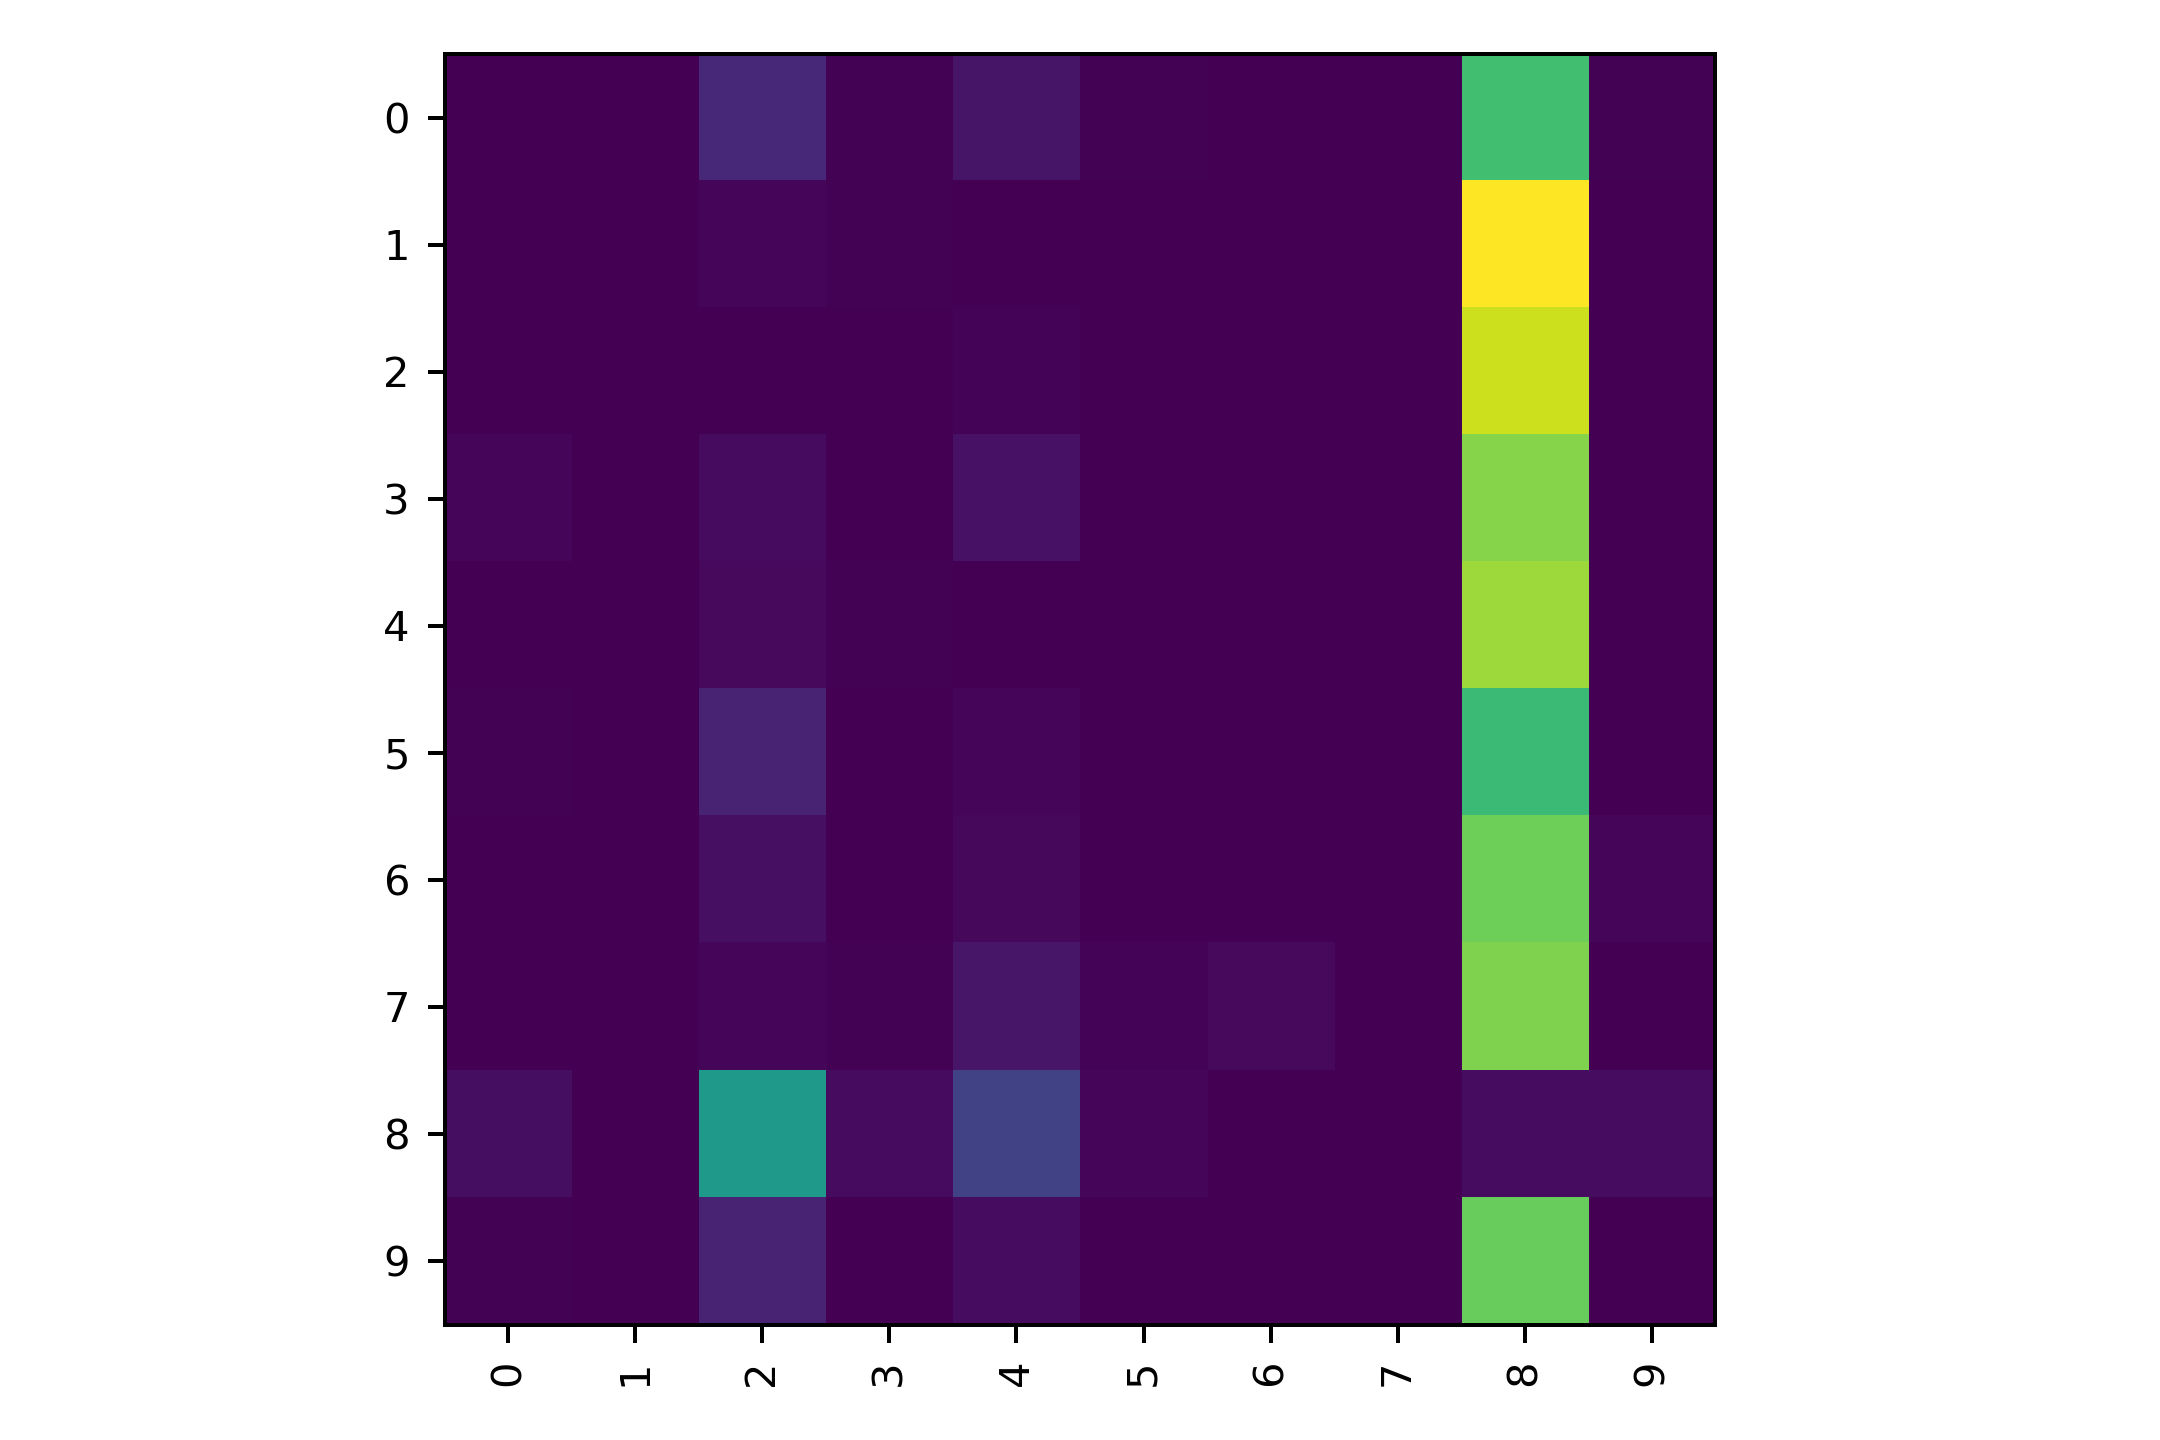
\includegraphics[align=c,width=0.3\columnwidth]{../code/results/MNIST/figures/LinfPGD, epsilon=1.png} &
	\end{tabular}
\end{frame}

\begin{frame}
	\frametitle{MNIST, $L^2$-Carlini-Wagner-Attack}
	
	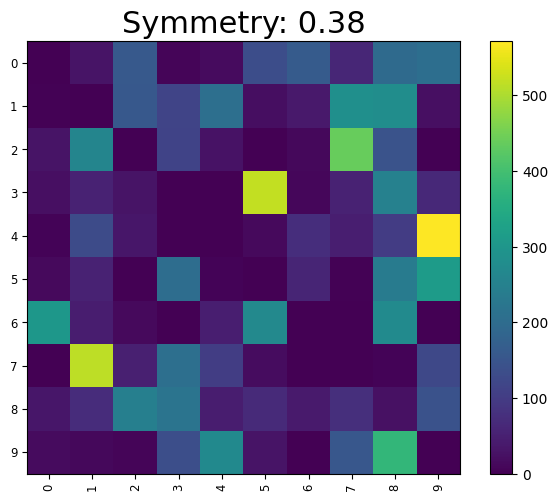
\includegraphics[align=c,width=0.9\textwidth]{../code/results/MNIST/figures/L2CarliniWagnerAttack.png}
\end{frame}

\begin{frame}
	\frametitle{CIFAR-10, $L^\infty$-PGD}
	\begin{tabular}{cccc}
		
		$\epsilon = 0.01$  & 	$\epsilon = 0.02$ & 	$\epsilon = 0.05$ & 	$\epsilon = 0.1$ \\
		
		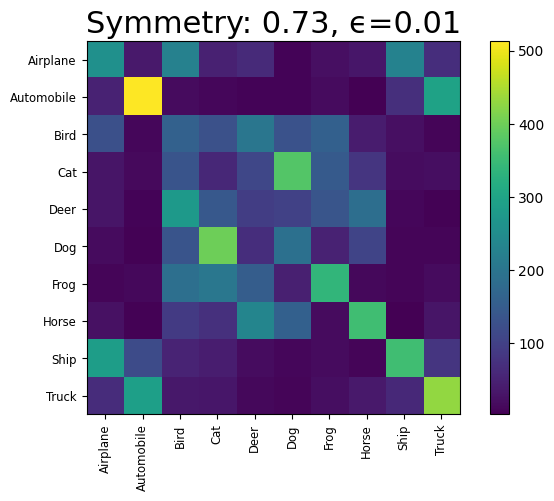
\includegraphics[align=c,width=0.3\columnwidth]{../code/results/CIFAR-10/figures/LinfPGD, epsilon=0.01.png} &
		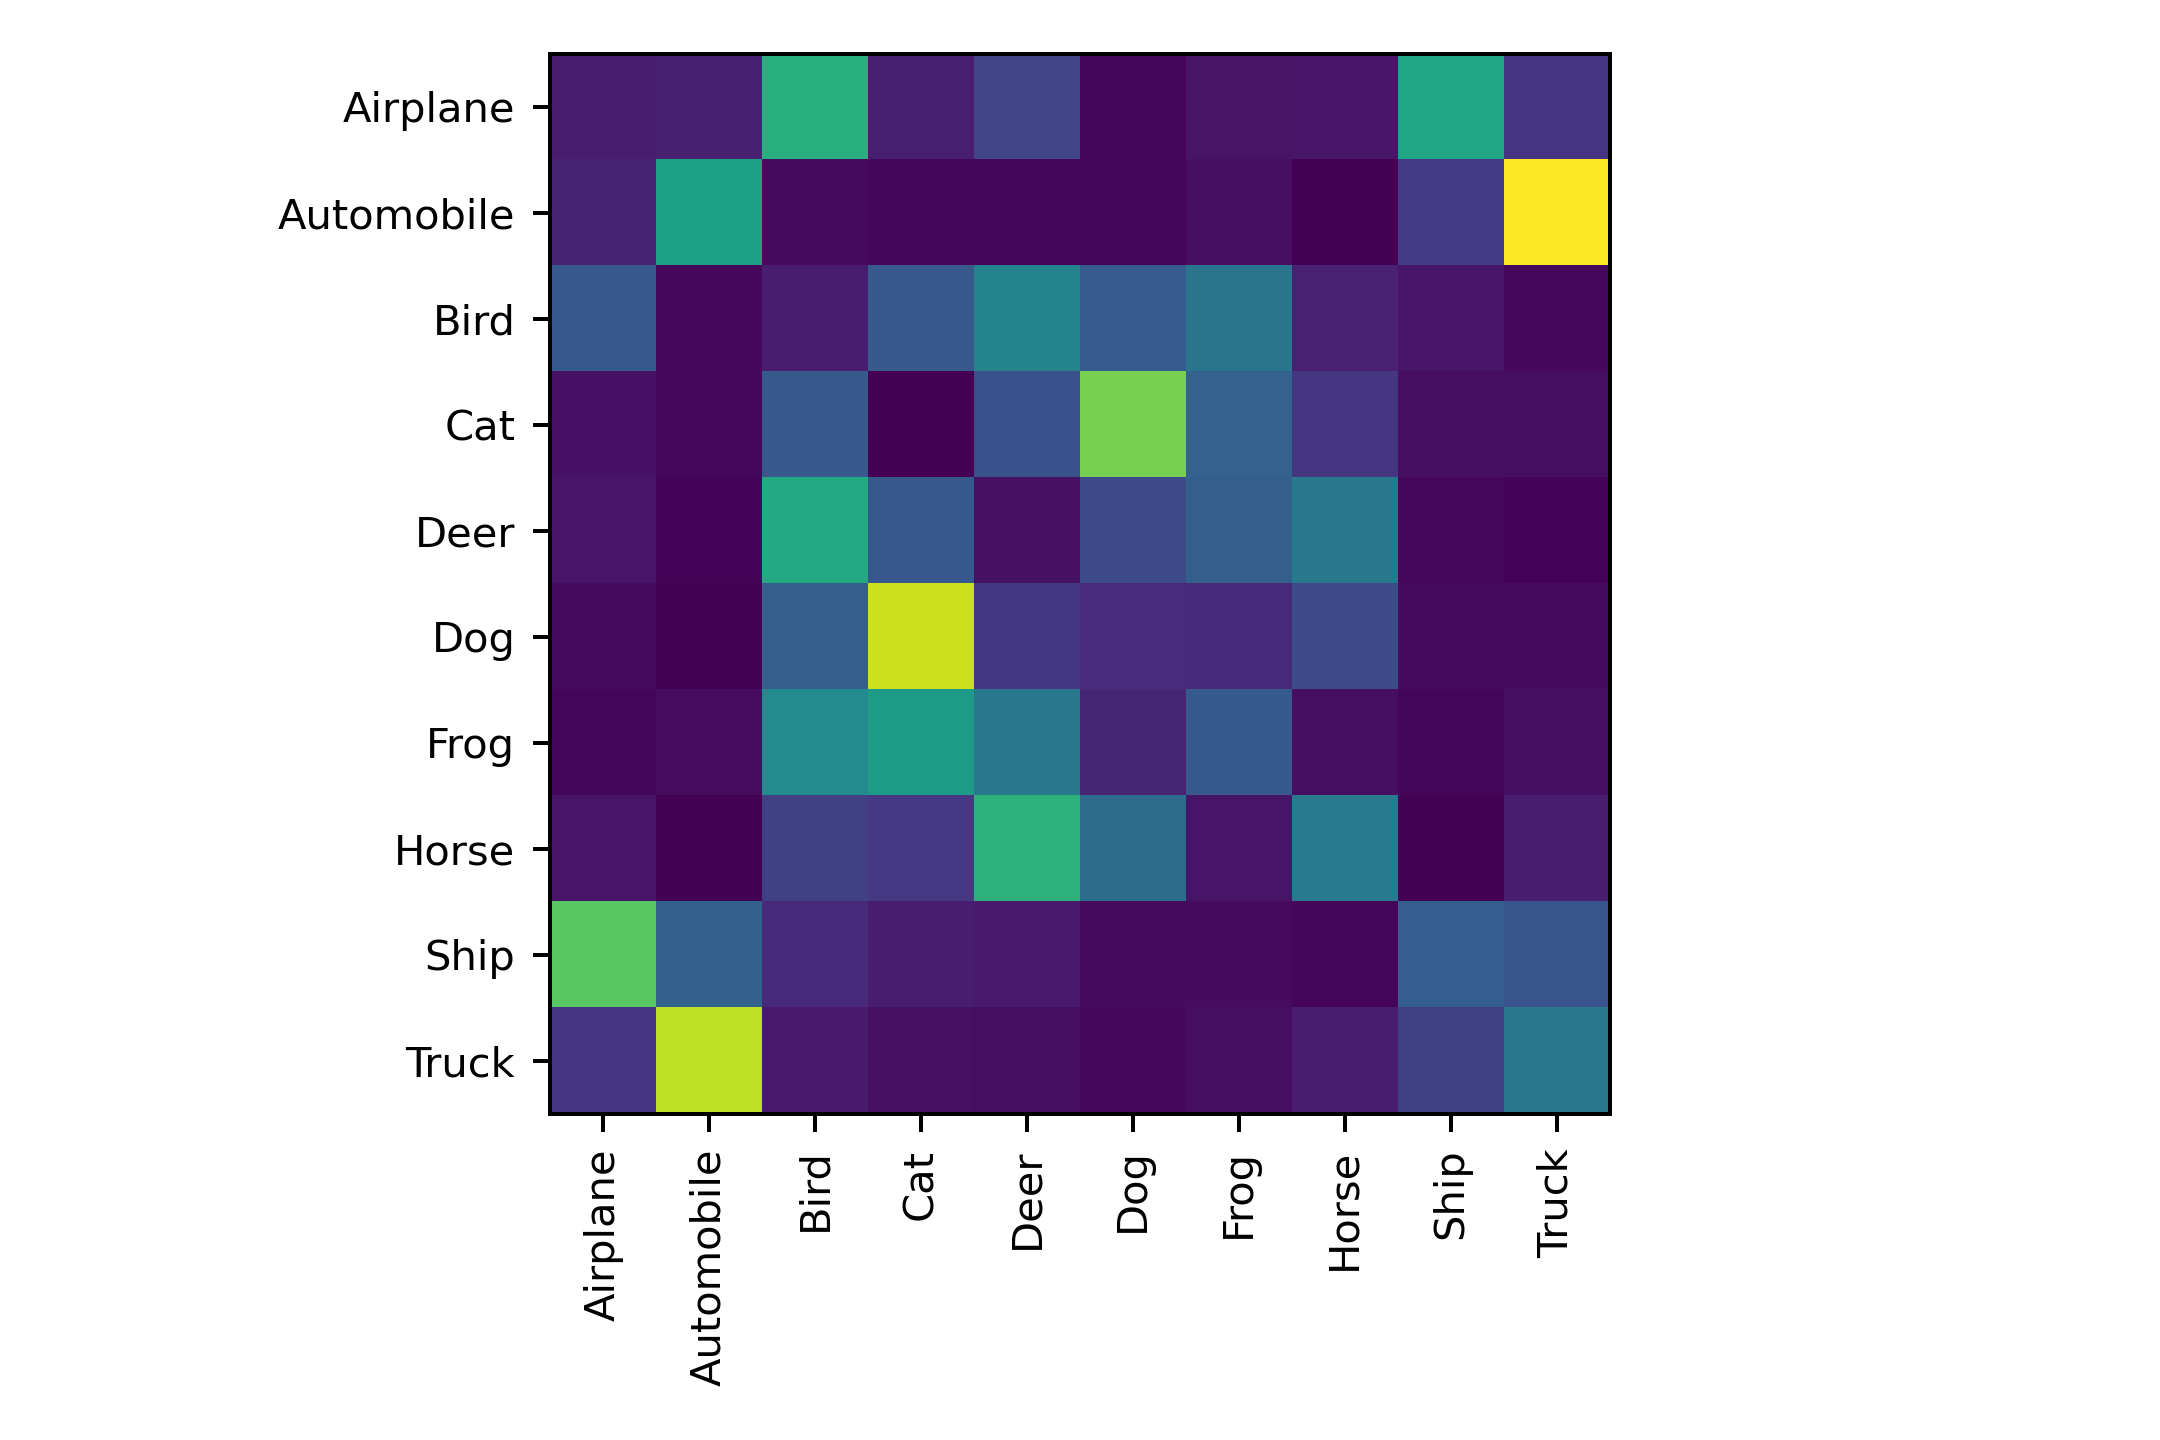
\includegraphics[align=c,width=0.3\columnwidth]{../code/results/CIFAR-10/figures/LinfPGD, epsilon=0.02.png} &
		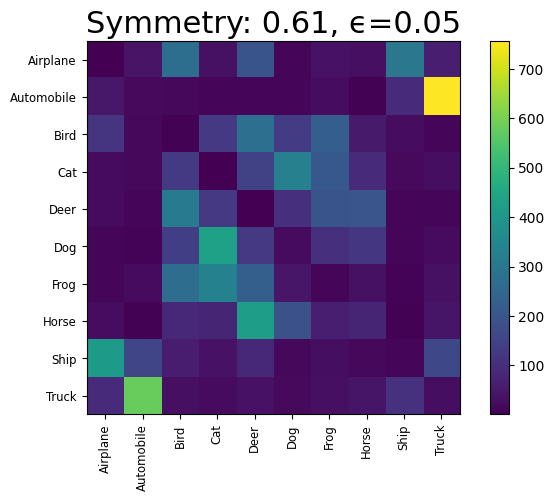
\includegraphics[align=c,width=0.3\columnwidth]{../code/results/CIFAR-10/figures/LinfPGD, epsilon=0.05.png} &
		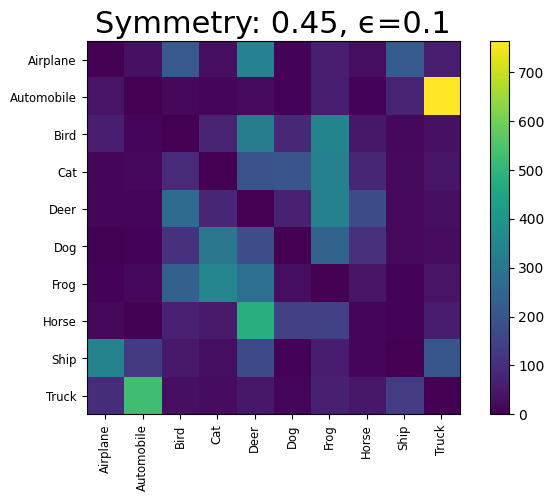
\includegraphics[align=c,width=0.3\columnwidth]{../code/results/CIFAR-10/figures/LinfPGD, epsilon=0.1.png} 
		\bigskip \\
		
		$\epsilon = 0.2$  & 	$\epsilon = 0.5$ & 	$\epsilon = 1$ & \\
		
		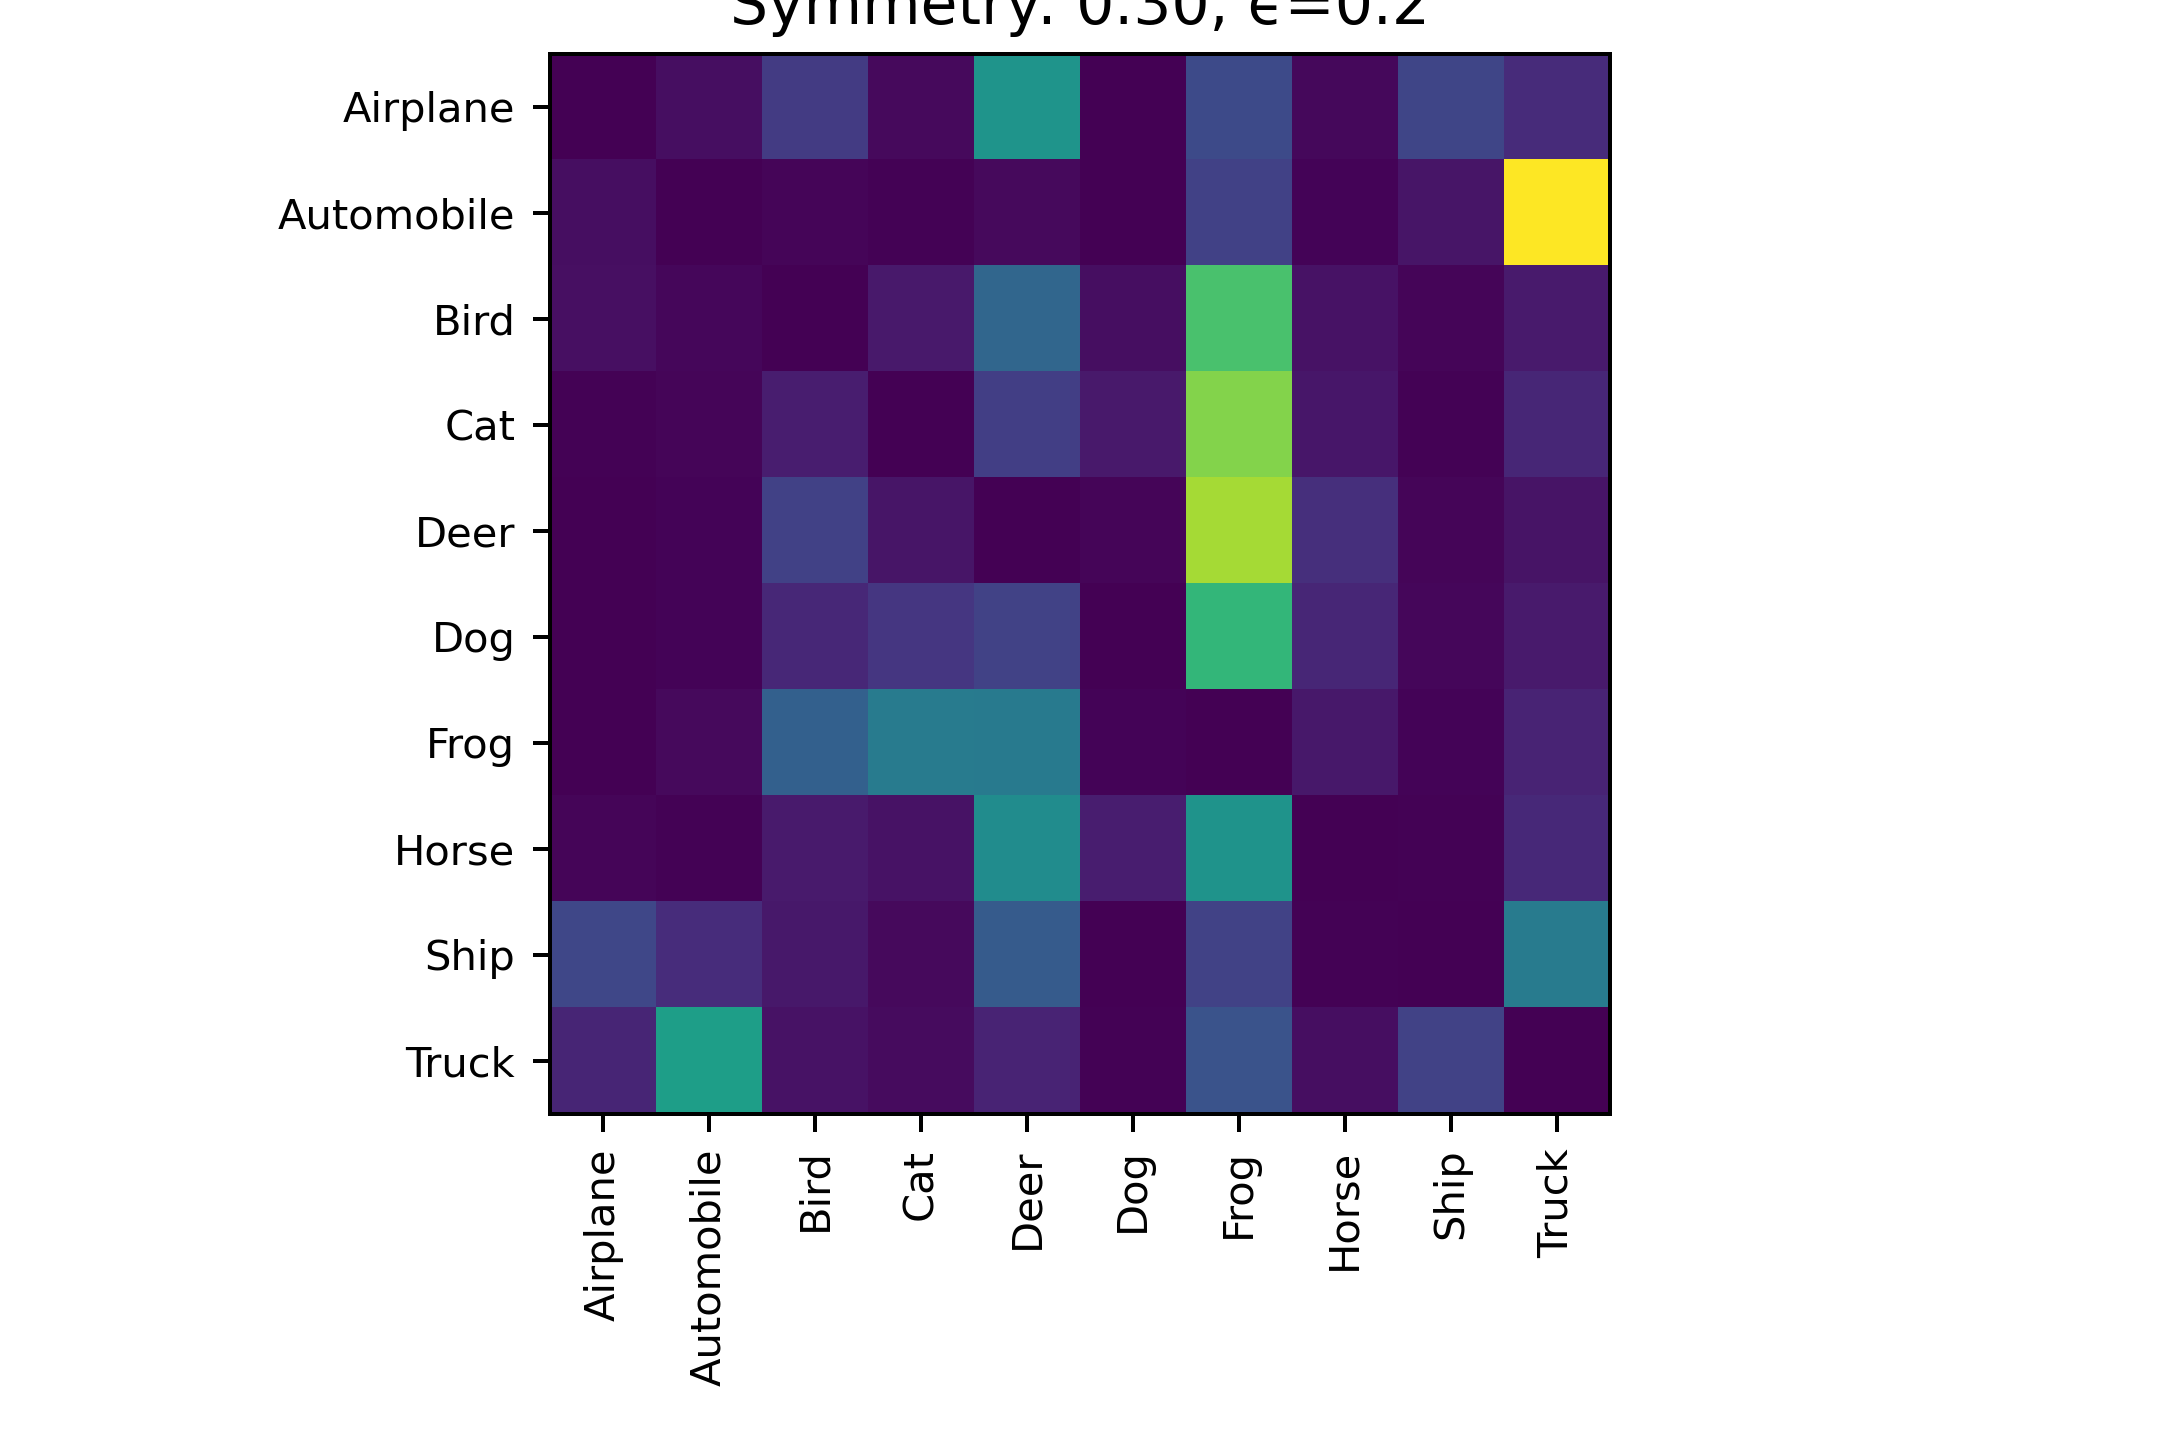
\includegraphics[align=c,width=0.3\columnwidth]{../code/results/CIFAR-10/figures/LinfPGD, epsilon=0.2.png} &
		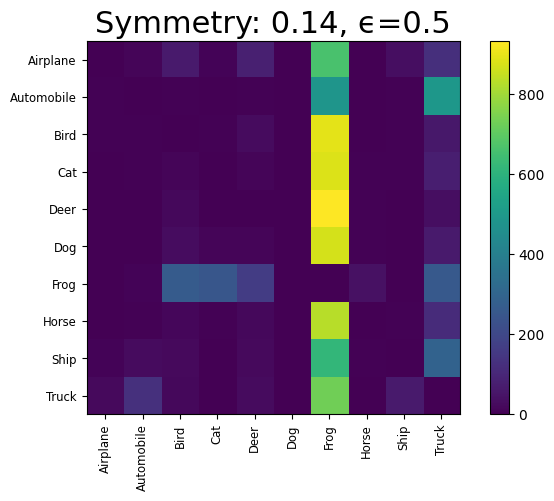
\includegraphics[align=c,width=0.3\columnwidth]{../code/results/CIFAR-10/figures/LinfPGD, epsilon=0.5.png} &
		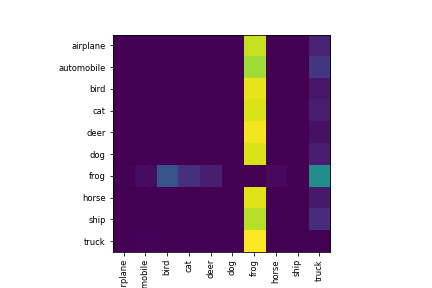
\includegraphics[align=c,width=0.3\columnwidth]{../code/results/CIFAR-10/figures/LinfPGD, epsilon=1.png} &
	\end{tabular}
\end{frame}

\begin{frame}
	\frametitle{CIFAR-10, $L^0$-Brendel-Bethge-Attack}
		
		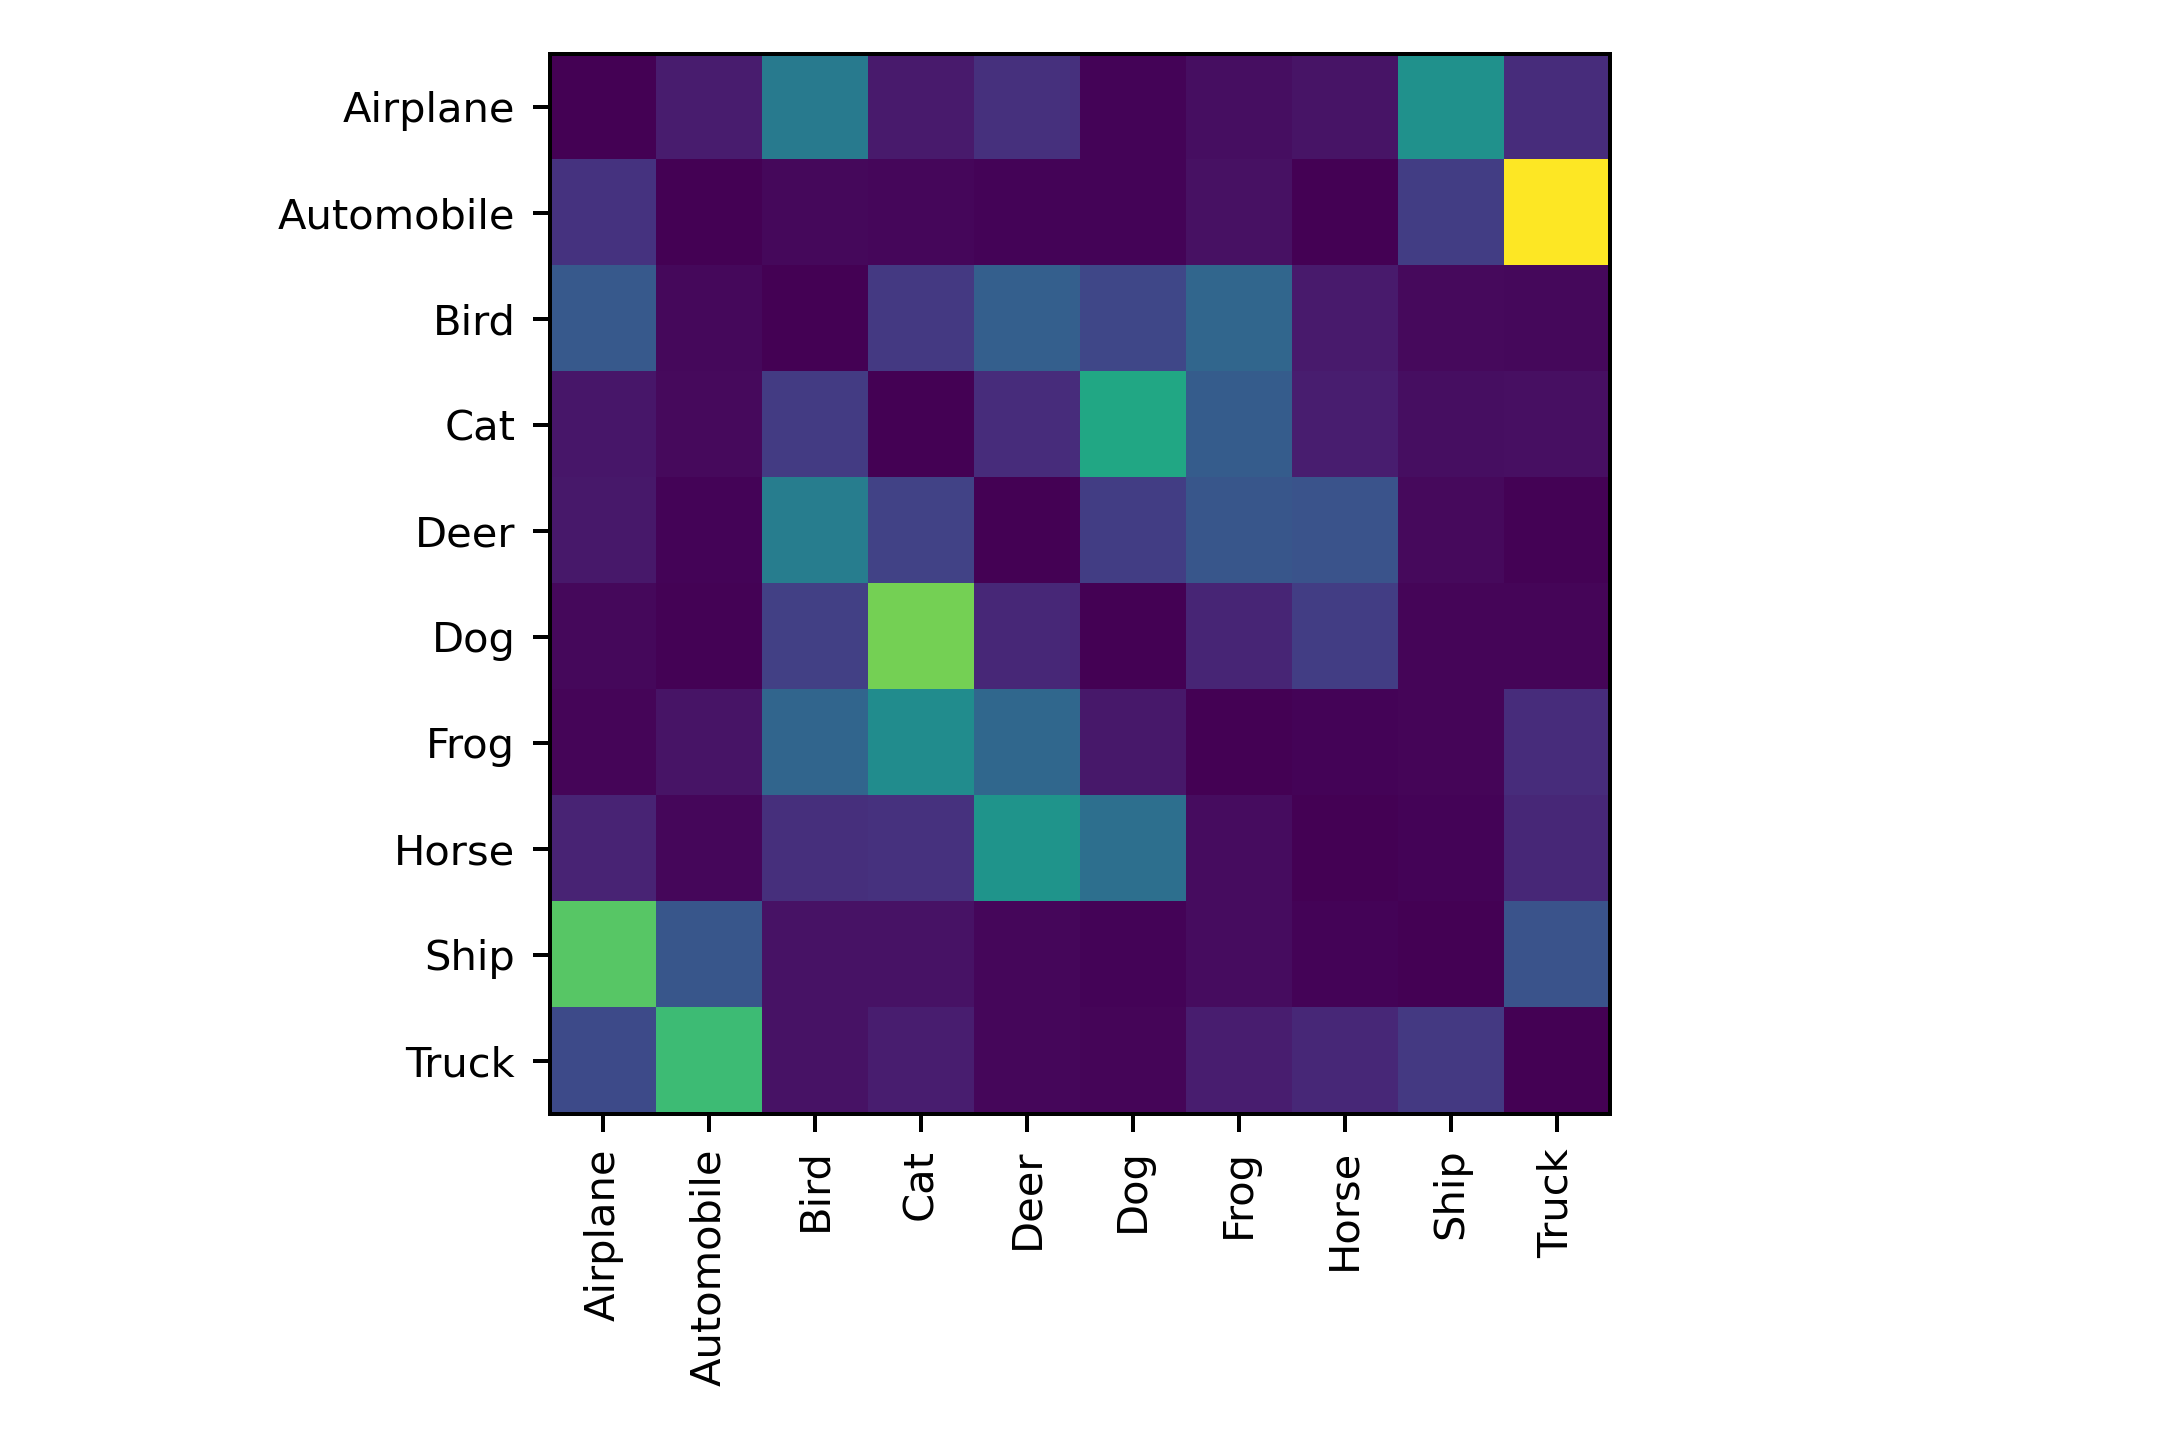
\includegraphics[align=c,width=0.9\textwidth]{../code/results/CIFAR-10/figures/L0BrendelBethgeAttack.png}
\end{frame}

\begin{frame}
	\frametitle{Tentative Findings}
	
	\large
	Small $\epsilon \rightarrow$ symmetric confusion matrix \\
	\medskip
	Large $\epsilon \rightarrow$ strong attractor classes ("8" and "frog")
\end{frame}

\begin{frame}[allowframebreaks]
	\frametitle{References}
	\bibliographystyle{unsrt}
	\bibliography{literature}
\end{frame}


\end{document}
